

\documentclass[]{beamer}
\setbeameroption{hide notes}
%\setbeameroption{show notes} %comment this away later
%\setbeameroption{show only notes}
\usepackage{pgfpages}
%\setbeameroption{show notes on second screen}
\mode<presentation>
{
  \usetheme{Warsaw}
  % or ...
  \setbeamercovered{transparent}

  % or whatever (possibly just delete it)
}
%\usepackage[square]{natbib}
\usepackage[english]{babel}
\usepackage[latin1]{inputenc}
\usepackage{amsmath, amsfonts, amssymb, xfrac}
\usepackage{subfig}
\usepackage{epstopdf}
%\usepackage{braket}
\usepackage{times}
\usepackage{tikz}
\usepackage{color}
%\usepackage[T1]{fontenc}
\usefonttheme[onlymath]{serif}

% Or whatever. Note that the encoding and the font should match. If T1
% does not look nice, try deleting the line with the fontenc.
\useoutertheme{infolines}
\usetikzlibrary{shapes.arrows}
\tikzset{
    myarrow/.style={
        draw,
        fill=blue,
        single arrow,
        minimum height=3.5ex,
        single arrow head extend=1ex
    }
}
\newcommand{\arrow}{%
\tikz [baseline=-0.5ex]{\node [myarrow] {};}
}
\newcommand{\mydownarrow}{%
\tikz [baseline=-0.5ex]{\node [myarrow, rotate=-90] {};}
}
\newcommand{\mybackarrow}{%
\tikz [baseline=-0.5ex]{\node [myarrow, rotate=-180] {};}
}


\graphicspath{ {./figures/} }
\newcommand {\be}{\begin{equation*}}
\newcommand {\ee}{\end{equation*}}
\newcommand{\ket}[1]{|#1\rangle}
\newcommand{\bra}[1]{\langle#1|}
\newcommand{\expect}[1]{\langle#1\rangle}
\newcommand{\braket}[2]{\langle#1|#2\rangle}
\newcommand{\ketbra}[2]{|#1\rlap{/}\backslash#2|}
\newcommand{\com}[1]{{\color{blue}#1}}

%to include movies
\usepackage{hyperref}
\usepackage{multimedia}
%use with pdfpc

\usepackage{listings}

\title[] % (optional, use only with long paper titles)
{Numerical integration of stochastic differential equations}
%\subtitle{Quantum noise in excitable laser systems} % (optional)
%
\author[] {Gerasimos Angelatos and  Zachary Hervieux-Moore
}
\institute[] {
\\[\medskipamount]
%\centering{
%\vspace{15pt}
%      \includegraphics[height=.25\textheight]{demofig.eps}%
%\vspace{-40pt}
%}
}
\date[] {} 


%
\subject{APC 523}
%% This is only inserted into the PDF information catalog. Can be left
%% out. 
%% If you have a file called "university-logo-filename.xxx", where xxx
%% is a graphic format that can be processed by latex or pdflatex,
%% resp., then you can add a logo as follows:
%\pgfdeclareimage[height=1.0cm]{university-logo}{QueensLogo_colour.png}
%\logo{\pgfuseimage{university-logo}}

% Delete this, if you do not want the table of contents to pop up at
% the beginning of each subsection:
%\AtBeginSubsection[]
%{
%  \begin{frame}<beamer>{Outline}
%    \tableofcontents[currentsection,currentsubsection]
%  \end{frame}
%}
%\AtBeginSection[]
%{
%  \begin{frame}<beamer>[noframenumbering]{Outline}
%    \tableofcontents[currentsection]
%
%  \end{frame}
%}

% If you wish to uncover everything in a step-wise fashion, uncomment
% the following command: 

%\beamerdefaultoverlayspecification{<+->}

\begin{document}
\AtBeginNote{\hspace*{-35pt} \begin{minipage}{1.15\textwidth} }
\AtEndNote{\end{minipage}}
%\setbeamerfont{note page}{size=\small}



\begin{frame}
 \titlepage
\end{frame}


\begin{frame}[noframenumbering]{Outline}
 \tableofcontents

\end{frame}

\section{Introduction}


\begin{frame}{Motivation}
%\begin{columns}
%\begin{column}{0.5\textwidth}

%\vspace{-10pt}
\begin{block}{Stochastic differential equations (SDEs}
\begin{itemize}
%  \setlength\itemsep{0.75em}
\item physics (quantum to astro), chemistry (melecular dynamics etc), probability theory, finance (Black-Scholes...)
\item Anything that evolves continuously and with some non-deterministic component
\end{itemize}
\end{block}
\begin{itemize}
  \setlength\itemsep{0.75em}
 \item Solution very different then for ODEs
\end{itemize}


%\end{column}
%\begin{column}{0.2\textwidth}
\begin{figure}[t]
\vspace{-1pt}
%\vspace{-2pt}
\captionsetup[figure]{labelformat=empty}
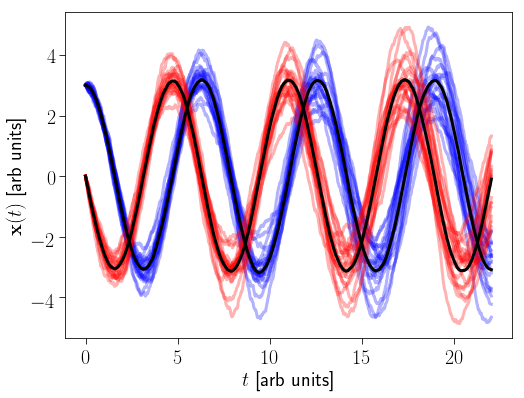
\includegraphics[width=0.4\textwidth]{sampleSDE.png}
\end{figure}
%\end{column}
%\end{columns}
\end{frame}


\subsection{Background}
\begin{frame}{Brownian motion: the Weiner process}
\begin{itemize}
  \setlength\itemsep{0.5em}
 \item White noise $\zeta(t)$: $\expect{\zeta(t)}=0$, uncorellated $\expect{\zeta(t)\zeta(t')}=\delta(t-t')$
\item Weiner process: $W(t)=\int_0^t ds \zeta(s)$
\end{itemize}

\be
p(W, t| 0, t_0)=[(2\pi)(t-t_0)]^{-\frac{1}{2}}e^{\frac{-W^2}{2(t-t_0)}} \label{eq:pwien}
\ee
\begin{columns}
\begin{column}{0.475\textwidth}
\begin{itemize}
%  \setlength\itemsep{0.75em}
 \item $\expect{{W}(t)}=0$,  $\expect{W(t)^2}=t-t_0$
\item Continuous
\item non-differentiable
\end{itemize}
\end{column}
\begin{column}{0.475\textwidth}
\begin{figure}[t]
\vspace{-20pt}
%\vspace{-2pt}
\captionsetup[figure]{labelformat=empty}
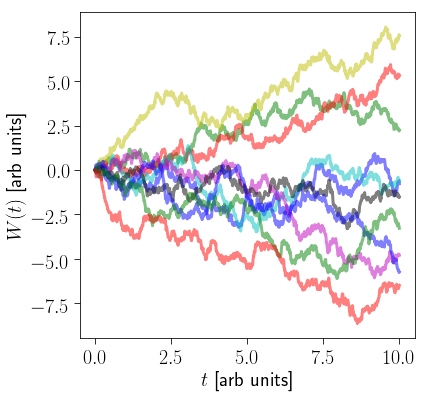
\includegraphics[width=0.8\textwidth]{Weiner.png}
\end{figure}
\end{column}
\end{columns}
\end{frame}

\begin{frame}{Stochastic differential equations}
\begin{itemize}
  \setlength\itemsep{1em}
 \item  Langavin equation: $\frac{d x}{dt}=A(x, t) +B(x, t)\zeta(t)$
\item SDE:  $x(t)=x(t_0)+\int_{t_0}^t A(x(s), s)+\int_{t_0}^t B(x(s), s) dW(s)$
\item $dW(t)=W(t+dt)-W(t)=\zeta(t)dt$
\item How to evaluate  $S=\int f(t')dW(t')$?
\item  $\lim_{n\to\infty}S_n$, \quad
$
S_n=\sum_i^n f(\tau_i)\left(W(t_i)-W(t_{i-1})\right),
$
\end{itemize}

\end{frame}


\begin{frame}{Ito Calculus}
\begin{itemize}
  \setlength\itemsep{1em}
 \item $S_n=\sum_i^n f(\tau_i)\left(W(t_i)-W(t_{i-1})\right)$
\item  $S_n$ depends on choice of $\tau_i$ in interval
\item Ito: $\tau=t_{i-1}$
\item $\expect{\int_{t_0}^t f(t')dW(t')}=0$
\item $dW(t)^2=dt $
\item Ito SDE: 
\end{itemize}
\be
d\mathbf{x}(t)=\mathbf{A}(\mathbf{x}, t)dt+\mathbf{B}(\mathbf{x}, t)d\mathbf{W}
\ee
\end{frame}

\section{SDE integration algorithms}
\begin{frame}{Explicit Euler}
\begin{itemize}
  \setlength\itemsep{1em}
 \item Discretize  $x(t_{k+1})=x(t_k)+\int_{t_k}^{t_{k+1}} A(x(s), s)ds+\int_{t_k}^{t_{k+1} } B(x(s), s) dW(s)$
\item $ \int_{t_k}^{t_{k+1}} dW(s)= W(t_{k+1})- W(t_{k})= \Delta W_k=\sqrt{\Delta t}\mathcal{N}(0,1)$
\end{itemize}
\begin{block}{Explicit Euler algorithm}
\be
 x_{k+1} = x_{k} + A(x_k, t_k)\Delta t +B(x_k, t_k) \Delta W_k
\ee

\end{block}
\end{frame}

\begin{frame}{Milstein}
\begin{itemize}
  \setlength\itemsep{1em}
 \item Explicit Euler  discards a term of order $\Delta t$
\item $\int_{t_k}^{t_{k+1}} \int_{t_k}^s dW(s)dW(s')=\frac{1}{2}\big(\Delta W_k^2-\Delta t\big)$
\item Inclusion gives Milstein:
\end{itemize}
\begin{block}{Milstein algorithm}
\begin{align}
C(x, t)=&\frac{1}{2}B(x,t)\partial_x B(x, t) \nonumber  \\
 x_{k+1} =& x_{k} + A(x_k, t_k)\Delta t +B(x_k, t_k) \Delta W_k+C(x_k, t_k) \big(\Delta W_k^2-\Delta t\big) \nonumber
\end{align}
\end{block}

\end{frame}

\begin{frame}{Semi-Implicit Euler}
\begin{itemize}
  \setlength\itemsep{1em}
 \item Implicit algorithms have far better stability
\item Stratonovich formulation: $S_n=\sum_i^n f(\frac{t_i +t_{i-1}}{2})\left(W(t_i)-W(t_{i-1})\right)$
\item Transform  $\mathbf{A}^{\rm strat}(x, t)=\mathbf{A}^{\rm Ito}(x,t)-C(x, t)$
\end{itemize}
\begin{block}{Semi-Implicit Euler algorithm}
\be
x_{k+1} = x_{k} + A^{\rm Strat}(\frac{x_{k+1}+x_k}{2},\frac{t_{k+1}+t_k}{2} )\Delta t +
B(\frac{x_{k+1}+x_k}{2}, \frac{t_{k+1}+t_k}{2}) \Delta W_k 
\ee
\end{block}
\end{frame}


\begin{frame}{Semi-Implicit Euler}

\begin{block}{Semi-Implicit Euler code}
\lstinputlisting[language=Python]{dummycode.py}

\end{block}
\end{frame}

\section{Convergence}

%then need a slide on convergence
\begin{frame}{Weak \& Strong Convergence}
There are two notions of convergence when it comes to SDE's. This is related to the different notions of convergence for probabilities.
\newline

\textbf{Weak Convergence:}
\begin{gather*}
  \left\lvert \mathbb{E} \left[ X_T \right] - \mathbb{E} \left[ X_T^{\delta t} \right] \right\lvert \leq O(\delta t)^\gamma
\end{gather*}

\textbf{Strong Convergence:}
\begin{gather*}
  \mathbb{E} \left[ \lvert X_T - X_T^{\delta t} \rvert \right] \leq O(\delta t)^\gamma
\end{gather*}

Where $\gamma$ is the rate of convergence of the different types.

\end{frame}

\begin{frame}{Weak \& Strong Convergence Differences}
\textbf{Weak Convergence:}
\begin{itemize}
  \item Similar to convergence in distribution
  \item Statement about the distribution's moments
  \item Useful for applications where we only care about the state of the system at the end point
\end{itemize}

\textbf{Strong Convergence:}
\begin{itemize}
  \item Analogous to convergence in the $L^1$ norm
  \item Strong statement about the paths themselves
  \item Important for applications where path matters such as Exotic Options pricing
\end{itemize}

\end{frame}

\section{Results}

\begin{frame}{Geometric Brownian Motion}
Geometric Brownian Motion is a famous model used in finance.
\begin{gather*}
    d S_t = \mu S_t dt + \sigma S_t d W_t
  \end{gather*}

  This process has multiplication noise and so it tends to be unstable. Furthermore, we know the solution of this SDE is
  \newline
  \textbf{Solution:}
  \begin{gather*}
    S_t = S_0 e^{(\mu - \frac{\sigma^2}{2})t + \sigma W_t}
  \end{gather*}
\end{frame}

%results slides!
\begin{frame}{Geometric Brownian Motion - Euler Scheme}
Expected Rate of Convergence: 1
\newline
Realized Rate of Convergence: 1
\begin{figure}[t]
\vspace{-1pt}
%\vspace{-2pt}
\captionsetup[figure]{labelformat=empty}
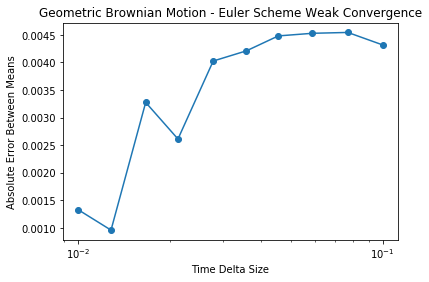
\includegraphics[width=0.4\textwidth]{gbm_euler.png}
\end{figure}
\end{frame}

\begin{frame}{Geometric Brownian Motion - Semi Implicit Euler Scheme}
Expected Rate of Convergence: 1
\newline
Realized Rate of Convergence: 1
\begin{figure}[t]
\vspace{-1pt}
%\vspace{-2pt}
\captionsetup[figure]{labelformat=empty}
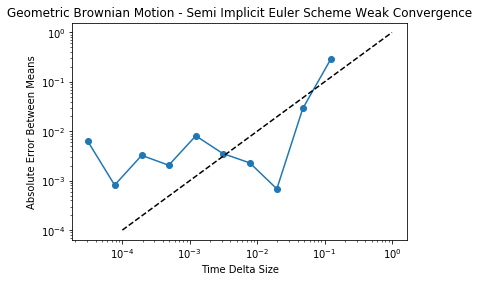
\includegraphics[width=0.4\textwidth]{gbm_semi.png}
\end{figure}
\end{frame}

\begin{frame}{Geometric Brownian Motion - Milstein Scheme}
Expected Rate of Convergence: 1
\newline
Realized Rate of Convergence: 1
\begin{figure}[t]
\vspace{-1pt}
%\vspace{-2pt}
\captionsetup[figure]{labelformat=empty}
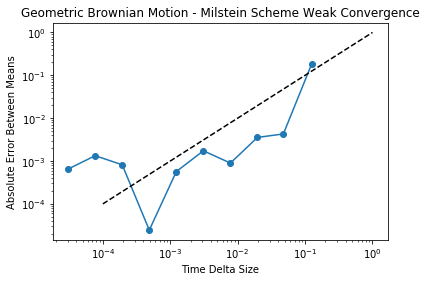
\includegraphics[width=0.4\textwidth]{gbm_milstein.png}
\end{figure}
\end{frame}

\begin{frame}{Ornstein-Uhlenbeck Process}
  The Ornstein-Uhlenbeck process is used to model biological systems as it is mean reverting.
  \begin{gather*}
    d X_t = \mu(\theta-X_t) dt + \sigma dW_t
  \end{gather*}

  This process differs from GBM in that the noise is only additive. Intuitively, this process tends towards $\theta$ as time goes on. The rate at which it tends there is dictated by $\mu$. The solution of the OU process is given by

  \begin{gather*}
    X_t = X_0 e^{-\mu t}+ \theta(1-e^{-\mu T}) + \sqrt{\frac{\sigma}{\mu} (1-e^{-2 \mu t})} W_t
  \end{gather*}

  Useful for us to consider because $\lvert X_T - X_T^{\delta t} \rvert$ has a closed form.
\end{frame}

\begin{frame}{Ornstein-Uhlenbeck - Euler Scheme}
  \begin{columns}
    \begin{column}{0.475\textwidth}
    \begin{center}
      \textbf{Weak Convergence}
    \end{center}
    \begin{figure}[t]
    \vspace{-1pt}
    %\vspace{-2pt}
    \captionsetup[figure]{labelformat=empty}
    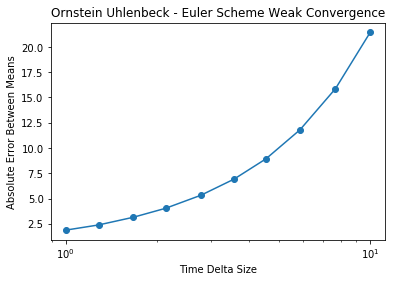
\includegraphics[width=0.4\textwidth]{ou_weak_euler.png}
    \end{figure}
    Theoretical Rate: 1
    \newline
    Realized Rate: 1
    \end{column}

    \begin{column}{0.475\textwidth}
    \begin{center}
      \textbf{Strong Convergence}
    \end{center}
    \begin{figure}[t]
    \vspace{-1pt}
    %\vspace{-2pt}
    \captionsetup[figure]{labelformat=empty}
    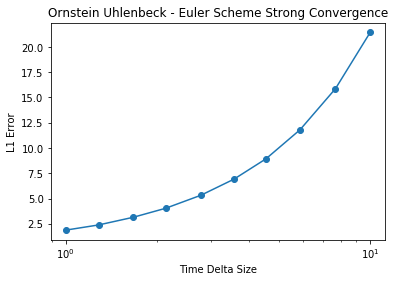
\includegraphics[width=0.4\textwidth]{ou_strong_euler.png}
    \end{figure}
    Theoretical Rate: 1/2
    \newline
    Realized Rate: 1
    \end{column}
  \end{columns}
\end{frame}

\begin{frame}{Ornstein-Uhlenbeck - Semi Implicit Euler Scheme}
  \begin{columns}
    \begin{column}{0.475\textwidth}
    \begin{center}
      \textbf{Weak Convergence}
    \end{center}
    \begin{figure}[t]
    \vspace{-1pt}
    %\vspace{-2pt}
    \captionsetup[figure]{labelformat=empty}
    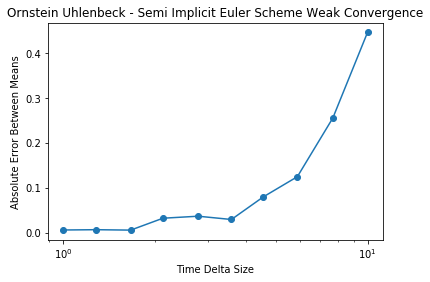
\includegraphics[width=0.4\textwidth]{ou_weak_semi.png}
    \end{figure}
    Theoretical Rate: 1
    \newline
    Realized Rate: 2
    \end{column}

    \begin{column}{0.475\textwidth}
    \begin{center}
      \textbf{Strong Convergence}
    \end{center}
    \begin{figure}[t]
    \vspace{-1pt}
    %\vspace{-2pt}
    \captionsetup[figure]{labelformat=empty}
    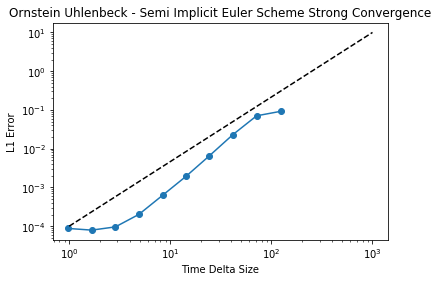
\includegraphics[width=0.4\textwidth]{ou_strong_semi.png}
    \end{figure}
    Theoretical Rate: 1/2
    \newline
    Realized Rate: 1
    \end{column}
  \end{columns}
\end{frame}

\begin{frame}{Ornstein-Uhlenbeck - Milstein Scheme}
  \begin{columns}
    \begin{column}{0.475\textwidth}
    \begin{center}
      \textbf{Weak Convergence}
    \end{center}
    \begin{figure}[t]
    \vspace{-1pt}
    %\vspace{-2pt}
    \captionsetup[figure]{labelformat=empty}
    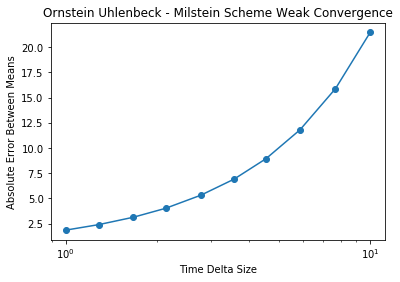
\includegraphics[width=0.4\textwidth]{ou_weak_milstein.png}
    \end{figure}
    Theoretical Rate: 1
    \newline
    Realized Rate: 1
    \end{column}

    \begin{column}{0.475\textwidth}
    \begin{center}
      \textbf{Strong Convergence}
    \end{center}
    \begin{figure}[t]
    \vspace{-1pt}
    %\vspace{-2pt}
    \captionsetup[figure]{labelformat=empty}
    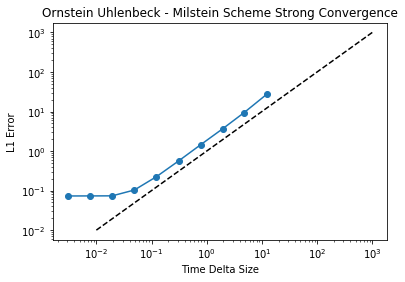
\includegraphics[width=0.4\textwidth]{ou_strong_milstein.png}
    \end{figure}
    Theoretical Rate: 1
    \newline
    Realized Rate: 1
    \end{column}
  \end{columns}
\end{frame}


\end{document}

